
\begin{table}[htbp]
%\resizebox{\textwidth}{!}
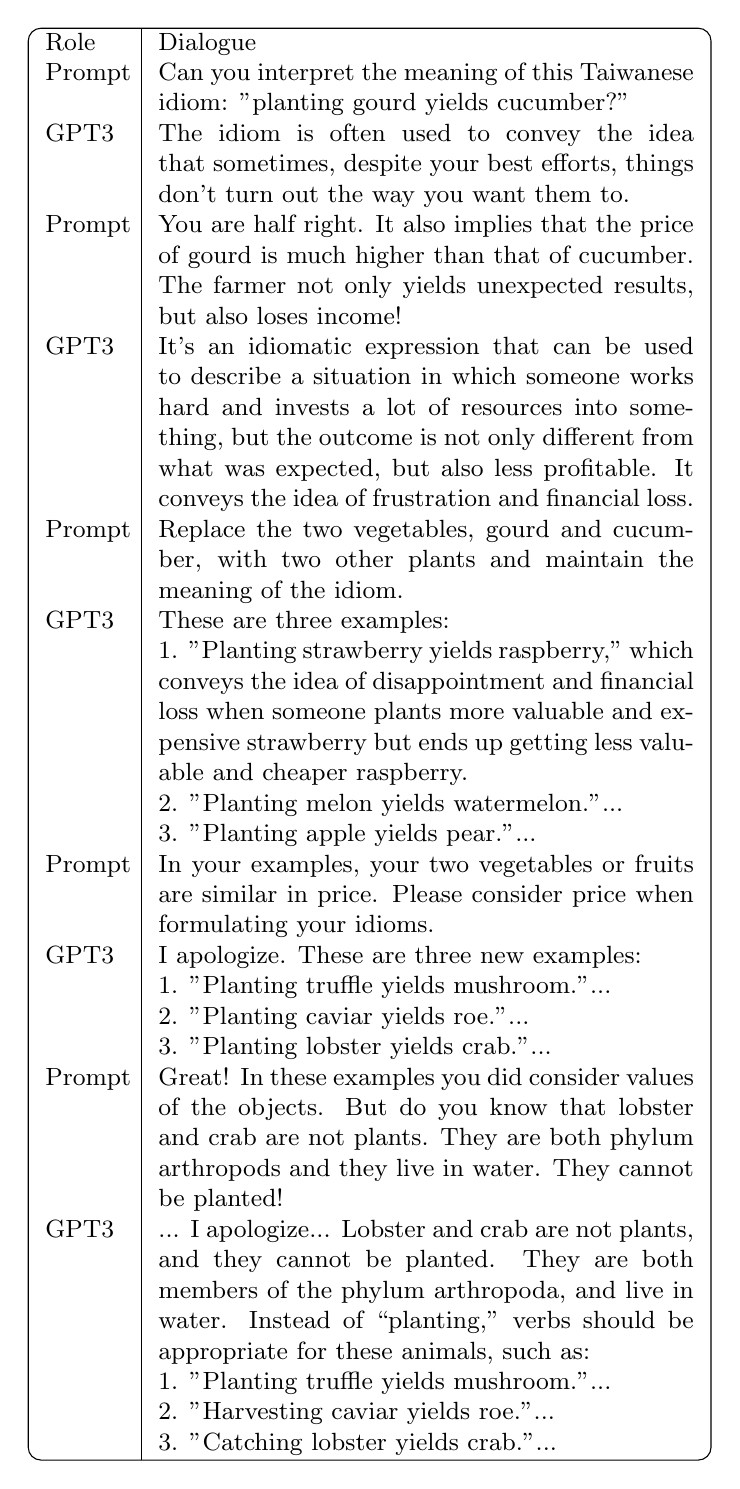
\begin{tikzpicture}
\begin{small}
\node (table) [inner sep=0pt] {
%\setlength\tabrowsep{1.5pt}
\begin{tabular}{p{1.0cm}|p{6.8cm}}
\toprule
Role & Dialogue \\
\midrule
Prompt & {Can you interpret the meaning of this Taiwanese idiom: "planting gourd yields cucumber?"}\\
GPT3 & {The idiom is often used to convey the idea that sometimes, despite your best efforts, things don't turn out the way you want them to.} \\
Prompt & {You are half right. It also implies that the price of gourd is much higher than that of cucumber. The farmer not only yields unexpected results, but also loses income! } \\

GPT3 & {It's an idiomatic expression that can be used to describe a situation in which someone works hard and invests a lot of resources into something, but the outcome is not only different from what was expected, but also less profitable. It conveys the idea of frustration and financial loss.} \\

Prompt & {Replace the two vegetables, gourd and cucumber, with two other plants and maintain the meaning of the idiom.} \\

GPT3 & {These are three examples:} \\
& 1. "Planting strawberry yields raspberry," which
conveys the idea of disappointment and financial loss when someone plants more valuable and expensive strawberry but ends up getting less valuable and cheaper raspberry. \\
& 2. "Planting melon yields watermelon."... \\
& 3. "Planting apple yields pear."... \\

Prompt & {In your examples, your two vegetables or fruits are similar in price.  Please consider price when
formulating your idioms.} \\

GPT3 & {I apologize. These are three new examples:} \\
& 1. "Planting truffle yields mushroom."... \\
& 2. "Planting caviar yields roe."... \\
& 3. "Planting lobster yields crab."... \\

Prompt & {Great! In these examples you did consider values of the objects. But do you know that lobster and crab are not plants. They are both phylum arthropods and they live in water. They cannot be planted! }  \\

GPT3 & {... I apologize... Lobster and crab are not plants, and they cannot be planted. They are both members of the phylum arthropoda, and live in water. Instead of ``planting,'' verbs should be appropriate for these animals, such as:} \\
& 1. "Planting truffle yields mushroom."... \\
& 2. "Harvesting caviar yields roe."... \\
& 3. "Catching lobster yields crab."... \\
\bottomrule
\end{tabular}
};
\draw [rounded corners=.5em] (table.north west) rectangle (table.south east);
\end{small}
\end{tikzpicture}
\caption{Example of Method Maieutics.}
\vspace{-.1in}
\label{tab:Maieutics}
\vspace{-.15in}
\end{table}
